\documentclass{beamer}

\mode<presentation> {
\usetheme{Madrid}
}

\usepackage{graphicx}
\usepackage{listings}
\usepackage{dirtytalk}
\graphicspath{{img/}}

\lstset{ basicstyle=\ttfamily\scriptsize}

\title[LLVM/Clang + Buildroot]{LLVM/Clang integration to Buildroot}

\author{Valentin Korenblit}
\institute[Smile]
{
Smile \\~\\
\medskip
\textit{valentin.korenblit@smile.fr}
}
\date{\today}

\begin{document}

\begin{frame}
\titlepage
\end{frame}

\begin{frame}
\frametitle{Overview}
\tableofcontents
\end{frame}

%-------------------------------------------------------
\section{Internship objectives}

\begin{frame}
\frametitle{Internship objectives}
\begin{itemize}
  \item Preliminary study of LLVM/Clang and OpenCL
  \item LLVM/Clang integration to buildroot
  \item OpenCL support for already existing packages in Buildroot (OpenCV, Mesa3D)
  \item Integration of new packages that can benefit from OpenCL: image processing (i.e. Darktable), simulation, cryptography, etc.
\end{itemize}
\end{frame}
%-------------------------------------------------------
\section{LLVM}

\begin{frame}
\frametitle{LLVM}
\begin{itemize}
  \item Open source project started in 2000
  \item Provides a compiler infrastructure written in C++
  \begin{itemize}
    \item Designed as an API from the beginning
    \item Focusing on compile time and performance of the generated code
  \end{itemize}
  \item Well structured and documented
  \item Some existing backends:
  \begin{itemize}
    \item \textbf{ARM}, ARM64, Hexagon, Mips, Mipsel, NVIDIA PTX 32/64, PowerPC 32/64, \textbf{AMD r600}, Sparc, Thumb, x86, \textbf{x86-64}, XCore
  \end{itemize}
\end{itemize}
\end{frame}

\begin{frame}[fragile]
\frametitle{LLVM - Internal aspects}
\begin{itemize}
  \item Intermediate Representation (IR)
  \begin{itemize}
    \item Architecture independent instruction set (RISC)
    \item Strongly typed
    \item Unlimited number of virtual registers in SSA
  \end{itemize}
  \item Optimizer
\end{itemize}

\begin{lstlisting}
      define i32 @main() #0 {
      entry:
        %retval = alloca i32, align 4
        %c = alloca i32, align 4
        store i32 0, i32* %retval, align 4
        %0 = load i32, i32* @a, align 4
        %1 = load i32, i32* @b, align 4
        %add = add nsw i32 %0, %1
        store i32 %add, i32* %c, align 4
        ret i32 0
      }
\end{lstlisting}

\end{frame}

\begin{frame}
\frametitle{LLVM - Three-phase approach}
\begin{figure}
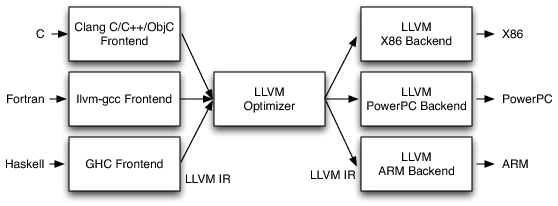
\includegraphics[width=0.8\linewidth]{img/llvm_struct.png}
\end{figure}
\end{frame}
%-------------------------------------------------------
\section{Clang}

\begin{frame}
\frametitle{Clang}
\begin{itemize}
  \item Frontend C/C++, Objective C/C++, OpenCL for LLVM
  \item Clear and concise diagnostics (error and warning messages)
  \item Macro expansion in error messages
  \item Sanitizers
  \item Goals
  \begin{itemize}
    \item Designed to be highly compatible with GCC
    \item Fully implement all ISO C++ standards until C++14 and most of C++17 (30 Nov 2017)
  \end{itemize}
  \item Performance vs GCC ?\footnote{\url{http://www.phoronix.com/vr.php?view=25742}}
\end{itemize}
\end{frame}
%-------------------------------------------------------
\section{Who is using LLVM/Clang}

\begin{frame}
\frametitle{Who is using LLVM/Clang}
\begin{itemize}
  \item Android: Renderscript compiler based on LLVM
  \item Apple
  \begin{itemize}
    \item All operating systems built with LLVM
    \item Xcode IDE uses Clang compiler and Clang static analyzer by default
  \end{itemize}
  \item FreeBSD can be entirely built with Clang/LLVM
  \item Google is using Clang for compiling their production builds of Chrome on Linux
  \item OpenCL: AMD, Apple, Intel, NVidia (runtime compiler)
  \item Sony Interactive Entretainment: CPU compiler for Playstation 4
\end{itemize}
\end{frame}
%-------------------------------------------------------
\section{Compiling Linux with Clang}

\begin{frame}
\frametitle{Compiling Linux with Clang}
\begin{itemize}
  \item Challenges
  \begin{itemize}
    \item Kernel expects to use some GCC behavior that is not supported by Clang:
    \begin{itemize}
      \item Variable Length Arrays inside structures
      \item Inline functions (GNU C extension)
      \item Explicit register variables
      \item LLVM assembler cannot be used to build the kernel
    \end{itemize}
  \end{itemize}
  \item LLVMLinux Project: Kernel 4.4 and 4.9 built with Clang for x86\_64 and ARM64 (need to apply some patches)\footnote{https://lwn.net/Articles/734071/}
  \item glibc ? binutils?
\end{itemize}
\end{frame}
%-------------------------------------------------------
\section{LLVM/Clang integration to Buildroot}

\begin{frame}
\frametitle{LLVM/Clang integration to Buildroot}
\begin{itemize}
  \item Existing work:
\end{itemize}
\end{frame}

\begin{frame}
\frametitle{LLVM/Clang integration to Buildroot - What it enables ?}
\begin{itemize}
  \item Gallium llvmpipe driver: software rasterizer that uses LLVM to do runtime code generation
  \begin{itemize}
    \item It is the fastest software rasterizer for Mesa3D
  \end{itemize}
  \item Applications that make use of OpenCL
\end{itemize}
\end{frame}

\begin{frame}
\frametitle{LLVM/Clang integration to Buildroot - Considerations}
\begin{itemize}
  \item LLVM/Clang versions
  \begin{itemize}
    \item Current version: 5.0.1 - Upcoming release: 6.0.0 on Feb 21
  \end{itemize}
  \item How to decide which packages are compiled with each compiler (GCC/Clang)?
  \begin{itemize}
    \item i.e. Debian packages: 28203 packages have been rebuild. Among them, 1445 (5.1 \%) failed \footnote{http://clang.debian.net/status.php?version=5.0}
  \end{itemize}
  \item Compile kernel with Clang?
  \item Which OpenCL implementation?
  \begin{itemize}
    \item {\fontfamily{qcr}\selectfont Clover}: used by Mesa. OpenCL 1.1 Supported, missing some OpenCL 1.2 functions
    \item {\fontfamily{qcr}\selectfont pocl}: many CPUs, ASIPs (TCE/TTA), NVIDIA GPUs (via CUDA). Approaching OpenCL 1.2 completeness in 2017
    \item {\fontfamily{qcr}\selectfont Beignet}: intel GPUs. Passed conformance for 1.2 in 2015, nearly complete OpenCL 2.0 in 2017
  \end{itemize}
\end{itemize}
\end{frame}
%-------------------------------------------------------
\begin{frame}
\Huge{\centerline{Thanks}}
\end{frame}

\end{document}
